% Number 700
% pTM Algebra Units Vectors
% Space probe thrust
% MIT/JG

% Watermark
\AddToShipoutPicture*{\BackgroundPic}

\addtocounter {ProbNum} {1}

\begin{floatingfigure}[r]{.55\textwidth}
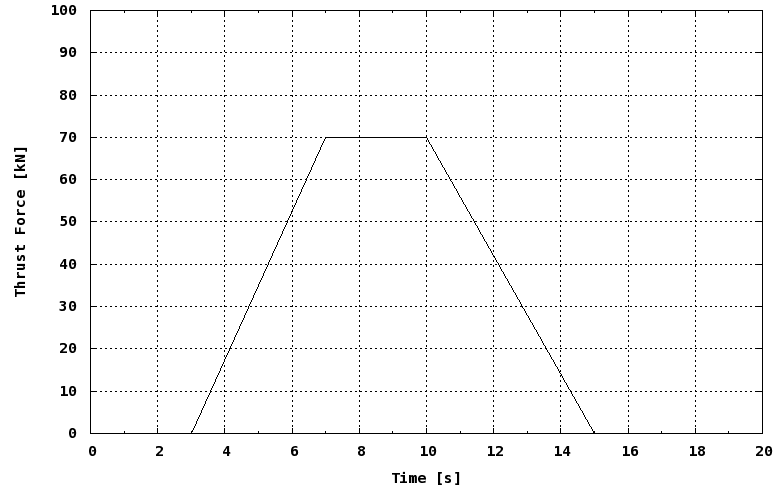
\includegraphics[scale=.4]{/Users/jgates/desktop/latex/pics/thrustgraph}
\end{floatingfigure}
 
{\bf \Large{\arabic{ProbNum}}} A space probe $(3870~kg)$ is flying with a speed of ${360~\tfrac{m}{s}}$. Thrusters are fired for a period of time, slowing down the probe, but not changing its direction. The plot shows the magnitude thrust force in kN during the firing sequence. 
\bigskip

Draw a diagram making it clear which direction the probe is moving and which direction the engine is pointing. What is the final speed of the probe?\paragraph{}
\noindent
\vfill

Draw, on the same set of axes, two graphs:
\MakeList{-}{
\item A \emph{velocity vs. time} graph for the probe, if instead a constant $50~kN$ thrust force is applied in the direction of the probe's motion, and...
\item a \emph{velocity vs. time} graph for the probe with the constant $50~kN$ thrust force from above, but taking into account the fact that the probe's mass decreases during the burn, as propellant is turned into gas which is shot from the engine. A qualitatively correct graph is all that you need here.}
\vfill
%\hfill 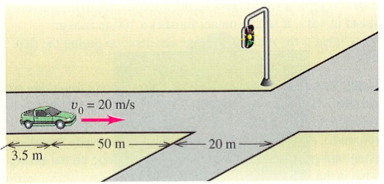
\includegraphics[scale=.85]{/Users/jgates/desktop/latex/pics/redlight.png}
\newpage
